\documentclass[tikz,border=10pt]{standalone}
\usetikzlibrary{calc,intersections}

\begin{document}
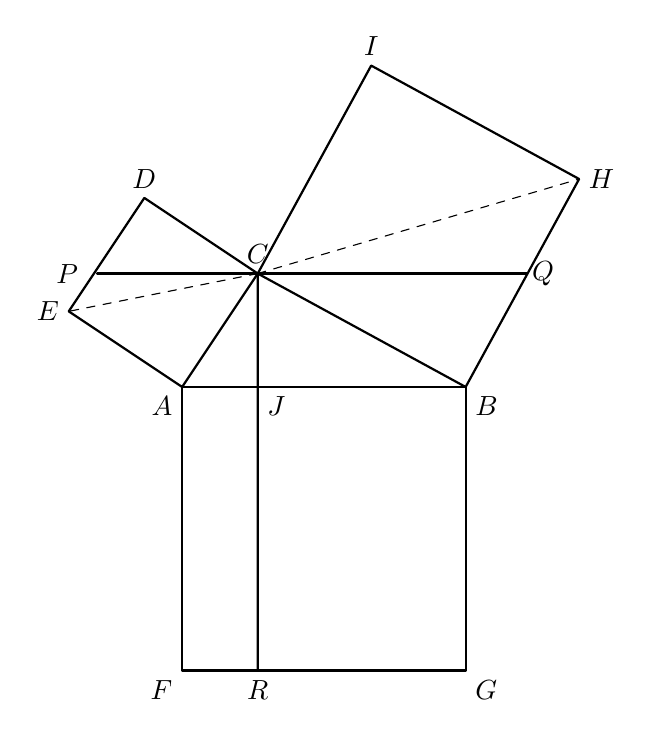
\begin{tikzpicture}[scale=1.2, line join=round, line cap=round]
    % --- 1. 定义核心点 ---
    % 设定三角形 ABC 的顶点，这里设为直角三角形（角C为直角）
    \coordinate (A) at (0, 0);
    \coordinate (B) at (3, 0);
    % 为了符合图像比例，设定 C 点坐标。可以通过勾股数设定一个比例
    \coordinate (C) at (0.8, 1.2); 

    % --- 2. 绘制下方的正方形 ABGF ---
    \coordinate (F) at (0, -3);
    \coordinate (G) at (3, -3);
    \draw[thick] (A) -- (B) -- (G) -- (F) -- cycle;

    % --- 3. 绘制左上的正方形 ACDE ---
    % 使用 calc 扩展计算旋转点
    \coordinate (D) at ($(C)!1!-90:(A)$);
    \coordinate (E) at ($(A)!1!90:(C)$);
    \draw[thick] (A) -- (C) -- (D) -- (E) -- cycle;

    % --- 4. 绘制右上的正方形 BCIH ---
    \coordinate (I) at ($(C)!1!90:(B)$);
    \coordinate (H) at ($(B)!1!-90:(C)$);
    \draw[thick] (B) -- (C) -- (I) -- (H) -- cycle;

    % --- 5. 绘制辅助线 ---
    % 过 C 点垂直于 AB 的直线（至正方形底边 FG）
    \draw[thick] (C) -- (0.8, -3) node[below] {$R$};
    \coordinate (J) at (0.8, 0); % 与 AB 的交点 J
    \node at (0.8, -0.2) [right] {$J$};

    % 水平辅助轴线 PQ (过点 C 且平行于 AB)
    \coordinate (P) at ($(E)!(C)!(D)$); % 点P在ED上
    \coordinate (Q) at ($(H)!(C)!(I)$); % 点Q在BH上
    \draw[dashed] (E) -- (P); % 补齐部分边
    \draw[thick] (-0.9, 1.2) -- (3.65, 1.2); % 过 C 的水平控制线
    \node[left] at (-1, 1.2) {$P$};
    \node[right] at (3.6, 1.2) {$Q$};

    % 斜向虚线 CE 和 CH
    \draw[dashed] (C) -- (E);
    \draw[dashed] (C) -- (H);

    % --- 6. 标注文本节点 ---
    \node[below left] at (A) {$A$};
    \node[below right] at (B) {$B$};
    \node[above] at (C) {$C$};
    \node[above] at (D) {$D$};
    \node[left] at (E) {$E$};
    \node[below left] at (F) {$F$};
    \node[below right] at (G) {$G$};
    \node[right] at (H) {$H$};
    \node[above] at (I) {$I$};

\end{tikzpicture}
\end{document}